\subsubsection{Launcher}

De zogenaamde launcher is het beweegbare compartiment waar alle Nerf darts in worden geladen
om af te schieten (zie bijlage \ref{app:launcher). Deze richt ook op de persoon.
De servo voor het tilt systeem wordt op het pan platform gemonteerd en met een arm aan de
launcher bevestigd. Dit wordt gedaan om de last op de servo te verminderen en de respons van
het systeem dus beter te maken. Ook wordt er aanbevolen om het scharnierpunt niet helemaal
achteraan te leggen zodat er een contragewicht is om nog meer last van de servo te halen.
Om het juiste montage punt van de arm van de servo te bepalen is er een serie driehoek berekeningen
nodig. Daarnaast kan er middels deze berekeningen ook de hoogte worden bepaald ten
opzichte van het pan platform (in verband met de neerwaartse beweging van het contragewicht).
Figuur \ref{fig:berrLauncher} toont een schematische weergave van het systeem. In deze figuur is $S_1$ de lengte van
het scharnierpunt tot de voorkant, $S_2$ is de lengte van het scharnierpunt tot de achterkant. $\alpha$ geeft
de maximale hoek aan van de launcher en $\delta/B$ is de uitslag van de achterkant ( de minimale hoogte
van de launcher).
Het bevestigingspunt van de arm van de servo op lengte $S_1$ ten opzichte van het kantelpunt kan
worden bepaald met de volgende formule.

\[P = \frac{2r}{\sin\alpha}\]

In deze formule is $r$ de lengte van de as tot het bevestigingspunt van de arm van de servo. Bij een
kruisvormige servo-arm zal deze afstand ongeveer 16 mm zijn. $P$ is het bevestiginspunt op lengte
$S_1$.

\begin{figure}
    \begin{center}
        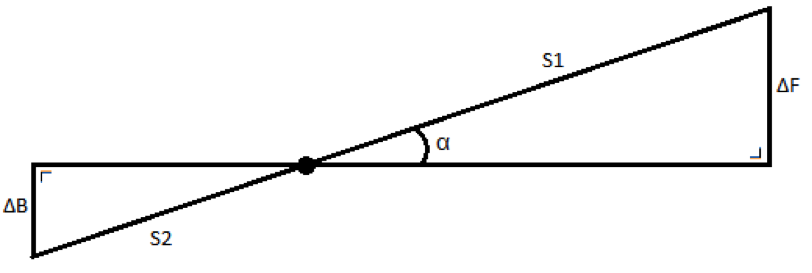
\includegraphics[scale=0.5]{figures/kantelpunt_launcher.png}
    \end{center}
    \caption{Schematische weergave servo montage punt.}
    \label{fig:berrLauncher}
\end{figure}

Door gebruik te maken van de bovenstaande formule is het mogelijk om de minimale montage hoogte van de
launcher te bepalen:

$\delta/B = S_2 \sin\alpha$

Bij het maken van deze berekening is het belangrijk rekening te houden met het bevestigingspunt
P zodat de servo niet te veel kracht moet zetten (dus niet te dicht bij het scharnierpunt). Daarnaast
is het belangrijk wel een goede hoek/actieradius te hebben. Dit is afhankelijk van de kijkhoek
van de camera en op welke afstand het systeem mensen moet kunnen herkennen/raken.
